\documentclass{article}

\PassOptionsToPackage{numbers, compress, sort}{natbib}
\usepackage[sglblindworkshop, final]{neurips_2026}
\workshoptitle{Predictive AI Evaluation Competition (PAIEC)}

\usepackage[utf8]{inputenc}
\usepackage[T1]{fontenc}
\renewcommand{\ttdefault}{lmtt}  % vector typewriter font (no bitmap Type 3 fonts)
\usepackage{hyperref}
\usepackage{url}
\usepackage{booktabs}
\usepackage{amsmath}
\usepackage{amsfonts}
\usepackage{nicefrac}
\usepackage{microtype}
\usepackage{xcolor}
\usepackage{graphicx}
\usepackage{multirow}
\usepackage{enumitem}

\hypersetup{colorlinks=true, linkcolor=blue!50!black, citecolor=blue!50!black, urlcolor=blue!50!black,
  pdftitle={LfHL: Learning from a Handful of Labels},
  pdfauthor={Arno Demarteau, Elias H\"uhne, Quentin Geoffroy}}
\setlist{leftmargin=1.5em, itemsep=1pt, topsep=2pt}

% The Codabench submission selected for the final evaluation.
\newcommand{\selectedid}{1038337}
% Name of the model (pooled_offset in the code).
\newcommand{\lfhl}{LfHL}
\newcommand{\repo}{\url{https://github.com/eliashuehne/paiec}}
\newcommand{\code}[1]{\texttt{#1}}
\newcommand{\labeled}{\code{labeled}}
\newcommand{\ALC}{\mathrm{ALC}}
\newcommand{\N}{\mathcal{N}}

\title{\lfhl: Learning from a Handful of Labels}

\author{%
  \normalfont $^{1}$Arno Demarteau, $^{1}$Elias H\"uhne, $^{1}$Quentin Geoffroy \\
  $^{1}$University of California, Berkeley
}

\makeatletter
\renewcommand{\@notice}{}
\makeatother

\begin{document}

\maketitle

\begin{abstract}
Predicting a system's performance on an unseen benchmark from only a handful of its answers is difficult, since information learned elsewhere transfers poorly. We examine which sources of information are useful for this task, using benchmark-held-out cross-validation on 1{,}720 system--benchmark pairs and the Brier area under the learning curve (ALC) of the Predictive AI Evaluation Competition. The text, metadata, tree-based and language-model features we tried improve ALC by about 0.001 or less. In contrast, a calibrated Bayesian update using a system's own labels reduces ALC from 0.25 to 0.2109, with other prior shapes providing almost no additional gain. Labels from other systems evaluated on the same benchmark provide another source of information. We introduce \lfhl{}, a hierarchical logistic model that pools a benchmark level, tag shifts and per-question shifts across systems. With 2, 5 and up to 20 systems, it achieves ALC scores of 0.2067, 0.2026 and 0.1968, respectively, with improvements in all five folds. Our ablation shows that learning the overall benchmark level accounts for most of the gain at low budgets, while question shifts become the main source of improvement at high budgets when many systems share a benchmark. These gains depend on the number of systems sharing a benchmark. Since development-platform runs score only eight or nine pairs, the gains with few systems are most relevant there. Identical uploads on the platform have a standard deviation of 0.0185, making single scores unreliable for ranking models. Our selected submission uses a calibrated \lfhl{} variant with update parameters fitted on public data.
\end{abstract}


\section{Introduction}
\label{sec:intro}

Evaluating every AI system on every benchmark is expensive, and many evaluation decisions only require a reliable estimate of system performance. Item Response Theory~\citep{Rasch1980,lord1980applications,lalor-etal-2016-building} and its recent applications to efficient evaluation~\citep{Rodriguez:Barrow:Hoyle:Lalor:Jia:Boyd-Graber-2021,polo2024tinybenchmarks} have shown that system ability and item difficulty can be estimated from a fraction of the responses \emph{within} a benchmark. The Predictive AI Evaluation Competition (PAIEC)~\citep{paiec2026} extends this problem to unseen benchmarks for which no training data is available. Specifically, the task is to predict $P(\text{correct})$ for each (system, question) using the question's text, system metadata, and $n \in \{0,1,3,7,15,31\}$ revealed answers.

However, benchmarks differ substantially in their formats, domains and definitions of a correct label. As a result, information learned from one benchmark does not necessarily transfer to another. This motivates the central question of our work: \emph{on a new benchmark, where does usable information come from?} We examine three available sources of information and find that their usefulness differs substantially (Figure~\ref{fig:sources}).


\begin{figure}[h]
  \centering
  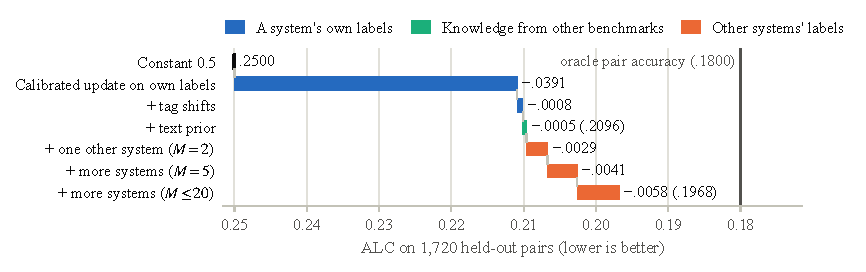
\includegraphics[width=\linewidth]{sources.pdf}
  \caption{Where usable information comes from on an unseen benchmark. Each step adds to the one above and shows its change in ALC, with the ALC reached in brackets where a source ends. Labels arrive from budget 1, and other systems' labels only if $M$, the number of systems of one benchmark whose labels are shared, exceeds one. Besides the text prior, the other features we tried from other benchmarks gain about 0.001 or less (Section~\ref{sec:before}).}
  \label{fig:sources}
\end{figure}

Our contributions are:
\begin{itemize}
  \item \textbf{A platform-faithful local evaluation} (Section~\ref{sec:protocol}). We implement benchmark-level five-fold cross-validation that reproduces the platform's split, nested budgets, shared \labeled{} lists and streaming acquisition. All learned parameters are fitted on training folds only.
  \item \textbf{An evaluation of the available information sources, including negative results} (Section~\ref{sec:results}). We examine what information transfers across benchmarks, how quickly the benefit from a system's own labels saturates, and what additional information other systems' labels provide.
  \item \textbf{\lfhl{}} (Section~\ref{sec:model}). We introduce a hierarchical logistic model that pools labels across systems and reduces to the own-label model when only one system is available. We further conduct an ablation of the shared terms to identify where the improvement comes from.
  \item \textbf{An analysis of the development platform conditions} (Section~\ref{sec:platform}). We examine how much of the pooling gain can be achieved on the platform and how little can be concluded from a single score.
\end{itemize}



\section{Task, data and evaluation protocol}
\label{sec:protocol}

A \emph{pair} consists of one system $s$ evaluated on one benchmark $b$ containing at least 80 distinct questions. The platform randomly divides each pair's questions into two equally sized pools, one for acquisition and one for evaluation. Acquisition candidates are presented sequentially, with an optional policy (\code{labeling.py}) determining which labels to reveal. Without such a policy, candidates are sampled uniformly. At each budget $n \in \{0,1,3,7,15,31\}$, the model predicts all evaluation questions using the labels revealed so far. The budgets are nested. Let $\mathrm{BS}_n$ denote the Brier score~\citep{Brier1950VERIFICATIONOF} at budget $n$. The score for each pair is
\begin{equation}
  \ALC = 0.1\,\mathrm{BS}_0 + 0.2\,(\mathrm{BS}_1 + \mathrm{BS}_3 + \mathrm{BS}_7 + \mathrm{BS}_{15}) + 0.1\,\mathrm{BS}_{31},
\end{equation}
which corresponds to the trapezoid rule on $\log_2(n+1)$. The overall suite score is the equally weighted mean across pairs, with constant predictions of 0.5 yielding 0.25. Repeated trials of the same question are treated as separate targets.

The organizers' ingestion code\footnote{\code{tools/streaming\_ingestion.py} of the official baseline repository (commit \code{cc88a95}), lines 147--181.} provides a \labeled{} list at each budget checkpoint, containing all labels purchased so far in the run. As a result, each target has access to the revealed answers of all other systems in the run, including systems evaluated on the same benchmark. These labels are available at the same budget as the target's own labels, but not at budget~0. However, both official baselines filter \labeled{} to retain only labels from the target system, leaving the remaining information unused.

\paragraph{Data.} We use only the public Measurement DB~\citep{measurementdb} for training, fixed at revision \code{54074453}. Of the 281 benchmark directories, 163 contain binary responses at the question level. We exclude three benchmarks marked \code{release = withheld}, leaving 160 benchmarks, of which 142 contain a total of 12{,}985 scoreable pairs. Three observations inform our design:
\begin{itemize}
  \item \emph{Systems rarely repeat}: 98\% of system ids appear in only one benchmark. The available system metadata is also sparse, with \code{normalized\_name} filled for 49\% of systems, release date for 33\%, and reasoning effort for 0.1\%. Furthermore, accuracy on another benchmark matched by system name correlates only 0.23 with accuracy on the target benchmark.
  \item \emph{Pairs differ a lot}: Pair accuracy has a mean of 0.54 and a standard deviation of 0.27. This corresponds to a spread of 1.62 on the logit scale, or 1.29 relative to each benchmark's mean.
  \item \emph{Questions do not recur across benchmarks}: Only 0.1\% of the 3.9\,M distinct public question texts appear in another benchmark, and none appear outside their own benchmark family.
\end{itemize}
We further calculate in-sample ceilings across all scoreable pairs to illustrate the differences between available information sources. Predicting each benchmark's mean achieves a Brier score of 0.217, compared with 0.174 when using each pair's accuracy and 0.133 when using each question's mean accuracy across systems.

\paragraph{Local evaluation.} We implement five-fold cross-validation using \code{scripts/run\_eval.py}, assigning the 160 benchmarks to folds with seed 0. For each fold, we fit all predictors from scratch on the other four folds and evaluate them on the held-out benchmarks. As a result, every benchmark is evaluated exactly once by a model that has not seen it during training. We select the first 20 pairs by system id from each benchmark and evaluate at most 200 questions per pair, resulting in 1{,}720 pairs across 142 benchmarks. Each pair is randomly divided 50/50 using a seed derived from (benchmark, system). Labels are then revealed in a seeded prefix of the acquisition order, following the platform procedure. To reproduce label pooling, we shuffle the pairs within each benchmark and divide them into \emph{pools} of $M$ systems. Every system in a pool is evaluated using the same shared list of revealed labels at budget $n$. We also simulate the streaming coordinator to evaluate acquisition policies. Since all methods are evaluated on identical pairs, we compare their performance using paired differences and report 95\% confidence intervals obtained through a bootstrap over benchmarks, accounting for correlations between pairs from the same benchmark. We additionally report the number of folds in which each candidate performs better. Our 286 unit tests include equivalence checks that verify, for example, that the fast vectorised scorers used during fitting agree with runtime predictions to $10^{-10}$.


\section{The model: \lfhl}
\label{sec:model}

For system $s$ answering question $q$ of benchmark $b$, \lfhl{} is
\begin{equation}
  \operatorname{logit} P(y_{sq}=1) = a_{sq} + \beta_b + u_s + \sum_{g \in G(q)} \gamma_g + v_q,
  \label{eq:pooled}
\end{equation}
\begin{equation*}
  \beta_b \sim \N(0, \rho\,\tau^2), \qquad u_s \sim \N\big(0, (1-\rho)\,\tau^2\big), \qquad \gamma_g \sim \N(0,\sigma^2), \qquad v_q \sim \N(0,\omega^2).
\end{equation*}

All terms beyond the starting logit $a_{sq}$ are learned from \labeled{} at prediction time. The benchmark level $\beta_b$, tag shifts $\gamma_g$ and question shifts $v_q$ are shared across systems with revealed labels on the same benchmark, while $u_s$ is specific to each system. The parameter $\rho$ determines how the pair-shift variance is divided between a shared benchmark level and a system-specific component. Question shifts provide information only when at least one system has revealed the corresponding question.

\paragraph{Own-label models are special cases.} When only one system is available, $\beta_b + u_s \sim \N(0,\tau^2)$ becomes a single pair shift $\delta_{sb}$. Removing the remaining terms gives the \emph{Bayesian offset}, $\operatorname{logit} P = \ell + \delta_{sb}$. Adding $\gamma_g$ produces \emph{tag shifts}, while replacing $\ell$ with a learned $a_{sq}$ gives the \emph{text prior}. With one system, \lfhl{} reproduces this model (tested to $10^{-9}$), except that revealed answers also affect evaluation questions with identical visible text. We additionally use the \emph{Beta-binomial} as a conjugate baseline, $p=(\alpha p_0 + k)/(\alpha+n)$ for $k$ correct answers out of $n$. This corresponds to the posterior mean under a Beta prior~\citep{efron1975data}.

\paragraph{Tag shifts.} Many benchmarks provide question-level tags in the form \code{key=value}, such as \code{task=qa3} and \code{lang=ja}. However, their meaning depends on the benchmark, making it difficult to transfer tag weights learned from training benchmarks. Instead, we estimate tag shifts from the revealed questions of the target benchmark. We select grouping keys using only the revealed questions (Appendix~\ref{app:details}). Tag values without revealed examples retain their prior variance $\sigma^2$.

\paragraph{Starting logit.} We train a logistic regression~\citep{scikit-learn} using hashed features~\citep{Weinberger2009Feature} from the information available to \code{predict}. These include 22 hand-made features and hashed tokens extracted from question text, tags and system fields. We weight pairs equally and select regularisation using held-out \emph{benchmarks}. The resulting logit $f_{sq}$ is incorporated as $a_{sq} = \ell + c + \lambda\,(f_{sq} - \mu)$, where the trust parameter $\lambda$ is learned from out-of-fold logits. Setting $\lambda = 0$ recovers a constant starting logit, allowing the text prior to contribute only when it improves performance on held-out data.


\paragraph{Inference.} For each benchmark in \labeled{}, we estimate a joint Laplace posterior~\citep{TierneyKadane1986} over $(\beta_b, u, \gamma)$ using Newton's method. We then estimate the question shifts $v_q$ separately in one dimension, keeping the other coefficients fixed. For each target, we sum the posterior means of its coefficients and calculate the variance from their posterior covariance, adding the prior variance of components not yet informed by revealed labels. We apply the probit approximation to the logistic--Gaussian integral~\citep{MacKay1992evidence}, $p = \sigma\big(m/\sqrt{1+\pi v/8}\big)$, which keeps early predictions close to the base rate. Questions are matched using their \emph{visible} content, consistent with the runtime interface. This matters because many benchmarks reuse the same prompt for questions that differ only in an attached file that the model cannot access. For example, one benchmark contains 2{,}960 questions but only 370 distinct texts.

\paragraph{Fitting.} We fit all parameters by minimising the training ALC over simulated episodes that reproduce the platform's split and reveal order on training benchmarks. First, we select $\ell$ and $\tau$ on a grid using the own-label offset. We then fit $(c,\lambda)$ and $(\tau,\sigma)$ using out-of-fold prior logits, followed by $\rho$ and $\omega$ on training benchmarks whose pairs are divided into pools of five. The search grids are provided in Appendix~\ref{app:details}. The fitted parameters remain stable across folds and agree with the observed data. In particular, $\tau = 1.58$ in every fold, compared with the measured logit spread of 1.62. We obtain $\sigma=0.75$ (0.5 in one fold), $\lambda \in [0.5, 1]$, and $\rho = 0.8$ and $\omega = 1.5$ in every fold. After training on all 160 benchmarks, the submitted parameters are $\lambda = 0.75$, $\tau=1.58$, $\sigma=0.75$, $\rho=0.8$, $\omega=1.5$.

\paragraph{Runtime.} Our submission uses only \code{numpy} and consists of \code{model.py}, four runtime modules and fitted parameters stored in a 0.5\,MB archive. It requires neither a pretrained model nor network access. Since all targets at a checkpoint receive the same \labeled{} list, we compute each benchmark's posterior once per list and cache the result.


\section{Results}
\label{sec:results}

\begin{table}[t]
  \caption{Five-fold cross-validated Brier score by budget and ALC on 1{,}720 pairs of 142 public benchmarks (lower is better), grouped by information source. $\Delta$: paired difference in ALC to the row above (for $M = 2, 5, \le 20$: to $M = 1$), with a 95\% bootstrap interval over benchmarks; folds: number of the five folds in which the row is better. The oracle row knows each pair's true accuracy on its evaluation questions.}
  \label{tab:main}
  \centering
  \footnotesize
  \setlength{\tabcolsep}{3pt}
  \begin{tabular}{@{}lccccccc@{\hspace{5pt}}l@{\hspace{4pt}}c@{}}
    \toprule
    Model & $\mathrm{BS}_0$ & $\mathrm{BS}_1$ & $\mathrm{BS}_3$ & $\mathrm{BS}_7$ & $\mathrm{BS}_{15}$ & $\mathrm{BS}_{31}$ & ALC & $\Delta$ ALC [95\% CI] & folds \\
    \midrule
    Constant 0.5 & .2500 & .2500 & .2500 & .2500 & .2500 & .2500 & .2500 & & \\
    \midrule
    Empirical mean (organizers) & .2500 & .3574 & .2412 & .2066 & .1941 & .1875 & .2436 & $-.0064$ [$-.0200$, $+.0059$] & 4 \\
    Beta-binomial & .2507 & .2301 & .2134 & .1998 & .1923 & .1871 & .2109 & $-.0327$ [$-.0372$, $-.0278$] & 5 \\
    Bayesian offset & .2505 & .2299 & .2133 & .1999 & .1924 & .1871 & .2109 & $-.0000$ [$-.0002$, $+.0001$] & 3 \\
    \quad + tag shifts & .2505 & .2299 & .2133 & .1991 & .1908 & .1842 & .2101 & $-.0008$ [$-.0012$, $-.0004$] & 5 \\
    \quad + text prior & .2494 & .2290 & .2127 & .1988 & .1907 & .1842 & .2096 & $-.0005$ [$-.0017$, $+.0007$] & 4 \\
    \midrule
    \lfhl, $M=1$ & .2494 & .2290 & .2127 & .1988 & .1907 & .1842 & .2096 & $|\Delta| < .0001$ (text twins) & -- \\
    \lfhl, $M=2$ & .2494 & .2241 & .2082 & .1962 & .1890 & .1827 & .2067 & $-.0029$ [$-.0038$, $-.0020$] & 5 \\
    \lfhl, $M=5$ & .2494 & .2151 & .2036 & .1930 & .1865 & .1799 & .2026 & $-.0070$ [$-.0088$, $-.0054$] & 5 \\
    \lfhl, $M\le 20$ & .2494 & .2055 & .1971 & .1886 & .1815 & .1734 & \textbf{.1968} & $-.0128$ [$-.0150$, $-.0106$] & 5 \\
    \midrule
    Oracle pair accuracy & .1800 & .1800 & .1800 & .1800 & .1800 & .1800 & .1800 & & \\
    \bottomrule
  \end{tabular}
\end{table}

\begin{figure}[t]
  \centering
  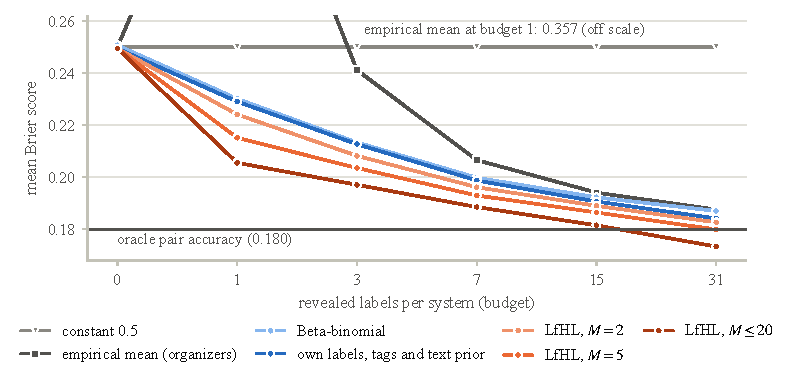
\includegraphics[width=\linewidth, trim=0 0 0 0, clip]{learning_curves.pdf}
  \caption{Mean Brier score by budget (same runs as Table~\ref{tab:main}). The naive empirical mean over-reacts to the first label (0.357 at budget 1, off scale). The Bayesian own-label models move smoothly; pooling labels across systems lowers every curve from budget 1 on, and with up to 20 systems it ends below the pair-accuracy oracle, which no own-label model can do.}
  \label{fig:curves}
\end{figure}


Table~\ref{tab:main} and Figure~\ref{fig:curves} show the progression. We take the three sources in the order in which they become available.


\subsection{Features from other benchmarks}
\label{sec:before}

The logistic text prior performs worse than a constant prediction of 0.5 when used on its own (Figure~\ref{fig:negative}). Furthermore, the regularisation selected on held-out benchmarks is the strongest in our grid for four of five folds. When incorporated into the own-label update, it improves ALC by only 0.0005, with an interval that includes zero. To investigate this result, we train the same features with a separate intercept for each pair, allowing the model to learn differences between questions rather than overall pair accuracy. On new questions from \emph{known} benchmarks, the model achieves an AUC of up to 0.66 (0.59--0.66 across regularisation strengths, 40 benchmarks). However, performance drops to 0.52 on an unseen fold. This suggests that surface features largely identify the benchmark rather than generalisable question difficulty. For example, 79\% of the variance in log question length occurs between benchmarks. The meaning of a correct label also differs across benchmarks, with some safety benchmarks treating a refusal as correct. We additionally evaluate gradient-boosted trees~\citep{NEURIPS2017_6449f44a} on the same features, allowing the model to capture system $\times$ question interactions. However, the fitting procedure assigns them less trust, and they perform worse than the logistic prior in four of five folds.

Two independent studies within our team support the same conclusion (Appendix~\ref{app:team}). The first evaluates system metadata using family-grouped folds, including release dates imputed for undated systems and identities recovered from model keys. None of the features improves ALC in four of five folds. Exact release dates even worsen performance ($+0.0025$), as they effectively identify individual systems. The second study evaluates a two-way ability $\times$ difficulty model against a model-free baseline that combines other systems' labels on the benchmark with the target pair's own labels. The model performs worse than the baseline (ALC 0.2036 against 0.2004), while its budget-0 predictions are also worse than a constant prediction of 0.5.

We further investigate whether language models can provide useful estimates of question difficulty. On 5{,}843 text questions from 40 benchmarks, we evaluate Qwen2.5-1.5B and 3B~\citep{qwen2025qwen25technicalreport} alongside two hosted models, gpt-4.1-mini and gpt-4.1 (Appendix~\ref{app:lm}). Each model rates the difficulty of individual questions. Even when given the benchmark's true level, these ratings explain only about 2\% of the remaining gap between a level-only prediction and a question oracle. The hosted models do not outperform the smaller models. However, this evaluation covers only a few models and one prompt, which we discuss further in Section~\ref{sec:limitations}.

\subsection{A system's own labels}
\label{sec:own}

\begin{figure}[t]
  \centering
  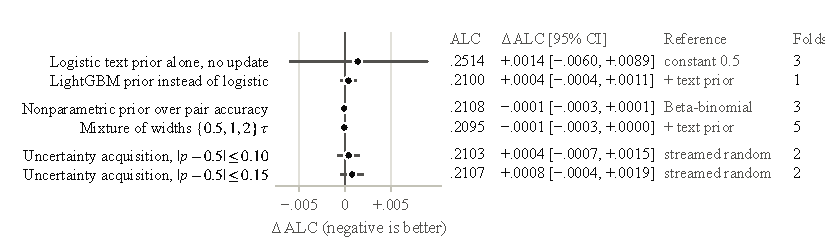
\includegraphics[width=\linewidth]{negative_results.pdf}
  \caption{Negative results under the same protocol (1{,}720 pairs): paired difference in ALC against the reference named in each row, with a 95\% bootstrap interval over benchmarks, and the number of folds where the row is better. Every interval includes zero. Streamed random acquisition, the reference of the last two rows, scores .2099 ($+.0003$ [$-.0010$, $+.0016$] against the fixed random order, one fold).}
  \label{fig:negative}
\end{figure}

\paragraph{Reacting to labels must be calibrated.} The organizers' empirical-mean baseline predicts accuracy directly from the revealed labels. After one label, this produces a prediction of either 0 or 1, resulting in a Brier score of 0.357 at budget 1, substantially worse than making no update. In contrast, any Bayesian update addresses this problem. The Beta-binomial outperforms the baseline on 75\% of pairs and in every fold ($-0.0327$), achieving a total gain of 0.039 over a constant prediction of 0.5. This represents by far the largest individual improvement in our results.

\paragraph{The update rule is saturated.} We compare three approaches to modelling pair accuracy: the Beta prior used by the Beta-binomial, the logit-normal prior of the Bayesian offset and a nonparametric kernel-density prior. All three achieve nearly identical ALC scores of 0.2108--0.2109. Furthermore, combining three prior widths in the full own-label model improves ALC by only 0.0001 (Figure~\ref{fig:negative}). The close agreement across four prior shapes suggests that the remaining error comes from the information available to the update rather than the choice of update rule. Tag shifts provide the only useful additional improvement ($-0.0008$, five of five folds, from budget 7 on). Unlike global tag weights, these shifts are estimated directly from the revealed questions of the target benchmark.

\paragraph{Label acquistion.} We evaluate an acquisition strategy that prioritises questions with predicted probabilities closest to 0.5. This corresponds to the official baseline's acquisition rule and a classic active-learning heuristic~\citep{settles.tr09}. However, it performs slightly worse than random sampling at both widths, with improvements in only two folds. With a single system, the main objective is to estimate the pair's overall level, for which any representative sample of labels is equally informative. Selecting questions based on their proximity to 0.5 under a weak text prior instead makes the sample less representative. Our simulation also allows skipped candidates to return at the next checkpoint, whereas the platform removes them from the stream. The acquisition policy is therefore more constrained on the actual platform. We submit no \code{labeling.py}.

\subsection{Other systems' labels}
\label{sec:others}

Sharing labels across systems evaluated on the same benchmark improves performance. With one other system, the gain is 0.0029; with five, it reaches 0.0070; and with up to 20, it increases to 0.0128, with improvements in all five folds and on 78\% of pairs. At budget 31, \lfhl{} with up to 20 systems achieves a score of 0.1734, outperforming the oracle that knows each pair's true accuracy (0.1800). This is impossible for a model that estimates only one number per pair. With one system, \lfhl{} reproduces the own-label results. Repeated question texts slightly affect 148 of 1{,}720 pairs, changing the mean by less than $10^{-4}$. As a result, pooling introduces no cost when \labeled{} contains no labels from other systems.

\begin{figure}[t]
  \centering
  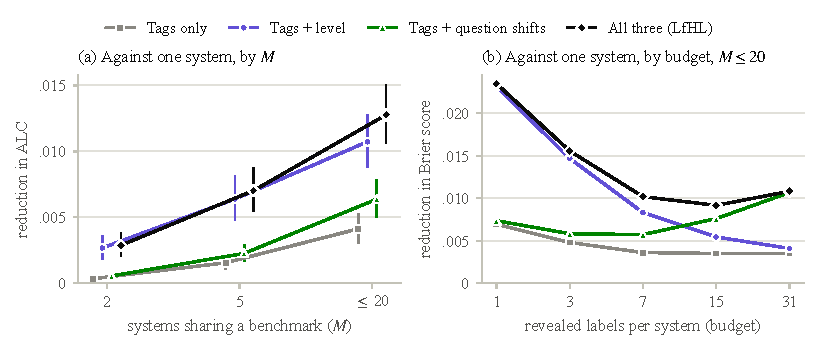
\includegraphics[width=\linewidth]{ablation.pdf}
  \caption{Pooling ablation: the same fitted models with shared terms switched off and nothing refitted. Tags stay on throughout because the one-system model uses them. (a) Reduction in ALC against \lfhl{} with one system (0.2096), with 95\% bootstrap intervals over benchmarks. (b) Reduction in Brier score at each budget with up to 20 systems: the benchmark level carries the gain early, question shifts late. Exact values are in Table~\ref{tab:ablation} (Appendix~\ref{app:details}).}
  \label{fig:ablation}
\end{figure}

\paragraph{Pooling ablation.} Figure~\ref{fig:ablation} shows the contribution of each shared term. The benchmark level accounts for most of the improvement across all values of $M$. Using only tags and the benchmark level retains 0.0027 of the 0.0029 gain at $M=2$, 0.0064 of 0.0070 at $M=5$, and 0.0107 of 0.0128 at $M \le 20$. In contrast, question shifts require another system to have revealed the same question. Their contribution is therefore small when few systems are available ($-0.0006$ at $M=2$, compared with $-0.0003$ for tags alone), but increases with $M$. The results across budgets further illustrate this difference. At budget 1 with $M \le 20$, the benchmark level reduces the Brier score from 0.2290 to 0.2059, compared with 0.2055 for the full model. Question shifts reach only 0.2217, compared with 0.2221 for tags alone. However, at budget 31, question shifts become more useful, achieving 0.1735 against 0.1734 for the full model. Tags and the benchmark level reach only 0.1801, close to the oracle that knows each pair's true accuracy (0.1800). These results show that other systems' labels initially provide information about overall benchmark difficulty, while at higher budgets they help identify which individual questions are difficult.

\paragraph{Why other systems can help.} Question difficulty is shared across systems evaluated on the same benchmark. We find that the mean accuracy of other systems on a question predicts whether a system answers it correctly with an AUC of 0.87 (sample of 40 benchmarks). A separate Rasch analysis (Appendix~\ref{app:team}) estimates question difficulty using one half of the systems on each benchmark and evaluates it on the remaining half. This achieves an AUC of 0.77, above chance on all 24 benchmarks tested. The analysis also shows that question difficulties vary considerably more than system abilities, with median standard deviations of 3.68 and 0.94 logits, respectively. In contrast, text features achieve an AUC of only 0.52 on unseen benchmarks.  This suggests that the difficulty of a question can be observed from other systems' answers more easily than it can be predicted from its text. However, this information is available only when another system has revealed the exact question. In the platform-sized draws of the Rasch analysis, this occurs for about one in nine evaluation questions even at budget 31.

\section{Selected submission}
\label{sec:platform}

Our selected Codabench submission \#\selectedid{} achieved a development Brier ALC of 0.133303. It uses the \lfhl{} variant with a starting probability of 0.35 before integrating over the offset, disables the text prior, and retains the update parameters fitted on public data. We tried this calibration in formative development. The submission uses random label acquisition. Table~\ref{tab:main} reports the default LfHL configuration. Development-platform runs score only eight or nine pairs in our logs, so the relevant gain there is that of $M=2$ (0.0029) rather than $M \le 20$ (0.0128). Identical uploads of one archive vary with a standard deviation of 0.0185 (47 uploads), so single scores cannot rank models. 

\begin{figure}[t]
  \centering
  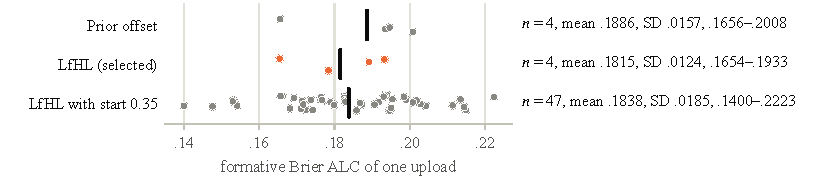
\includegraphics[width=\linewidth]{uploads.pdf}
  \caption{Formative Brier ALC of our own uploads. Each row is one unchanged archive uploaded repeatedly; dots are uploads and bars are means, and the right column gives the number of scored uploads, the mean, the standard deviation and the range. The prior offset uses own labels and the text prior; the last archive has no text prior, and five further uploads of it finished without a score.}
  \label{fig:uploads}
\end{figure}

\section{Limitations}
\label{sec:limitations}

\begin{itemize}
  \item \textbf{Overlap between systems.} Our pooled evaluation assumes a fixed number $M$ of systems per benchmark. However, the number of systems in the final test is unknown, and the improvement depends on how many systems share a benchmark (Section~\ref{sec:platform}).
  \item \textbf{Public versus platform pairs.} We fit all parameters on public benchmarks, which also determine the starting level of our selected model. Platform scores (Figure~\ref{fig:uploads}) and budget-0 results suggest that the hidden pairs differ from the public data. As a result, improvements observed locally may not transfer directly to the platform.
  \item \textbf{Local protocol.} We group our cross-validation folds by benchmark rather than benchmark family (e.g.\ the ten \code{medhelm\_*} benchmarks). Since our improvements primarily come from labels revealed at test time rather than learned features, this should have little effect, although family-grouped folds would provide a stricter evaluation. To reduce computational cost, we evaluate at most 20 pairs per benchmark and 200 questions per pair, using a single seed for splits and folds. The platform does not publish its candidate order, so we simulate the acquisition process.
  \item \textbf{Ablation.} We disable individual terms without refitting the remaining parameters, preventing them from compensating for the removed components. Tag shifts are also included in every row.
  \item \textbf{Question-level information.} The question oracle achieves a score of 0.133, substantially below the performance of our models. Pooling captures only part of this information, since it requires other systems to have revealed the same questions. None of the information sources we tested provides more than marginal transfer for a single system. However, we did not evaluate sentence embeddings or open models with tens of billions of parameters, and our predictor does not use a language model. Our language-model study is limited to 40 benchmarks, four models and one rating prompt. Larger models or different prompts may capture considerably more information.
  \item \textbf{Team studies.} The additional studies in Appendix~\ref{app:team}, apart from the prior variants, use separate evaluation protocols, so the AUCs compared in Section~\ref{sec:others} are not directly comparable. Furthermore, our within-pair diagnostics of the text prior cover only one fold.
\end{itemize}

\section{Conclusion}
\label{sec:conclusion}

Our results show that on unseen benchmarks, the most useful information comes from revealed labels rather than features learned from other benchmarks. A calibrated update of a single shift per pair captures most of the information provided by a system's own labels, with four different prior shapes showing that further improvements are limited. In contrast, labels from other systems provide additional information about the benchmark's overall difficulty and, as more labels become available, the difficulty of individual questions. \lfhl{} uses this information when other systems are available, while reducing to the own-label model when they are not. These findings suggest that, for evaluation design, increasing the overlap between systems on a benchmark may be more useful than developing a more complex predictor. Beyond the proposed model, we hope that our evaluation protocol, negative results and analysis of score noise will also be useful for future work.

{\small
\bibliographystyle{plainnat}
\bibliography{references}
}

\newpage
\appendix

\section{Reproducing the results}
\label{app:repro}

\paragraph{Reproducibility.} We release the code, tests and scripts used to generate the tables and figures at \repo{} (branch \code{main}). Appendix~\ref{app:repro} provides the commands, run times and seeds. We verify the reproducibility of our submission from a fresh clone, successfully completing installation, all 286 tests and both archive builds. The official checker accepts the resulting archives. The rebuilt default archive matched the earlier upload (\#1019997), with identical code apart from line endings and fitted arrays differing by at most $3 \times 10^{-14}$. The rebuilt \code{start035} archive matched the supplied archive for the selected variant, with identical fitted arrays and Python code apart from line endings. This verification uses an existing copy of the data rather than downloading it again. We additionally re-run the pooled model at $M=2$ using the ablation script and find that all reported numbers remain unchanged, with the largest difference on a single score being $1.2 \times 10^{-4}$ and the mean ALC difference remaining below $10^{-6}$.

All commands run from the repository root with Python 3.10 (\code{numpy}, \code{pandas}, \code{pyarrow}; \code{scikit-learn}, \code{scipy} and \code{lightgbm} for training; \code{matplotlib} for the figures). The data download needs a Hugging Face account with access to the gated Measurement DB.

\begin{footnotesize}
\begin{verbatim}
git clone https://github.com/eliashuehne/paiec && cd paiec
git submodule update --init  # baseline at cc88a95
python -m venv .venv && source .venv/bin/activate    # or .venv\Scripts\activate
pip install -e ".[dev]" matplotlib
hf auth login && python scripts/download_data.py     # revision 54074453, ~5 GB
python -m pytest                                     # 286 tests

# Table 1, Figures 1-2 (five folds, seed 0; 0.5-3 h per command on a laptop CPU)
python scripts/run_eval.py --predictors constant empirical_mean shrunk_mean \
    offset tag_offset
python scripts/run_eval.py --predictors prior_offset gbdt_offset logreg_prior
python scripts/run_eval.py --predictors pooled_offset --pool-sizes 1 2 5 all
# Figure 3, acquisition rows
python scripts/run_eval.py --predictors prior_offset --acquisition-items 100 \
    --policies random uncertainty10 uncertainty15
# Figure 4, Table 2 and the start-0.35 variant (about 35 min, one process per fold)
python scripts/run_pooling_ablation.py --folds 0 1 2 3 4
python scripts/run_pooling_ablation.py --merge

# Selected archive (training on all 160 benchmarks: 11-15 min)
python scripts/train_submission.py      # artifacts/pooled_offset.npz
python scripts/calibrate_submission.py --start 0.35 --no-text-prior
python scripts/build_submission.py --artifacts artifacts/pooled_offset_start035.npz \
    --zip dist/pooled_offset_start035.zip

# Numbers and figures of this report (set the run folders in RUNS first)
python report/make_figures.py
\end{verbatim}
\end{footnotesize}

{\raggedright In the code, \lfhl{} is the predictor \code{pooled\_offset}. Each run of \code{run\_eval.py} writes per-pair scores to \code{runs/<timestamp>/pairs.csv}. From these, \code{report/make\_figures.py} computes the bootstrap intervals (4{,}000 resamples of benchmarks, seed 0) and the figures, and writes \code{report/results/numbers.json}. The data facts of Section~\ref{sec:protocol} and the diagnostics of Section~\ref{sec:before} come from \code{scripts/analysis/}, the language-model pilot from \code{scripts/pilot/}. The nonparametric prior of Figure~\ref{fig:negative} is on branch \code{logreg} (commit \code{aa0f0b2}); the mixture and budget-0 prior variants are on branch \code{model/subject-features-enhanced} (commit \code{39f93d2}) as predictors \code{mix\_prior\_offset} and \code{zero\_prior\_offset}. All experiments ran on one laptop (Intel Core Ultra 9 185H, 32\,GB RAM); only the language-model pilot used its GPU (NVIDIA RTX 4060 Laptop).\par}

\section{Implementation details}
\label{app:details}

\paragraph{Episodes.} Fitting replays the platform protocol on training benchmarks: for at most 20 randomly chosen pairs per benchmark (each benchmark contributes at most 20 pairs of weight), the pair's questions are split with the same seeded 50/50 rule, the first 31 acquisition questions are the revealed labels, and at most 200 evaluation questions are scored. Every candidate parameter value is scored by the exact ALC of these episodes, with vectorised implementations that the tests check against the runtime code.

\paragraph{Grids.} Own-label offset: 31 levels in $[-1.5, 1.5]$ $\times$ 41 values of $\tau$ in $[0.1, 10]$ (log-spaced). Beta-binomial: 81 values of $\alpha$ in $[0.05, 200]$. Text prior: $c \in \{-0.2, 0, 0.2\}$ $\times$ $\lambda \in \{0, 0.25, 0.5, 0.75, 1, 1.5\}$ at $\sigma = 0.75$, then $\tau \times \{0.7, 0.85, 1\}$ $\times$ $\sigma \in \{0.5, 0.75, 1\}$. Pooling: $\rho \in \{0, 0.2, 0.35, 0.5, 0.65, 0.8, 0.9, 0.95\}$ $\times$ $\omega \in \{0, 0.5, 1, 1.5, 2, 3\}$ on pools of five. Logistic regularisation $C \in [0.003, 1]$ chosen on an inner 20\% of training benchmarks ($C = 0.01$ in the submission).

\paragraph{Tag keys.} A key is used if it has at least four revealed questions, two or more values and repeating values; long or hash-like values are dropped.

\paragraph{Features.} Item: log characters, words and lines; digit and non-ASCII share; code, mathematics, JSON, question mark, empty content; detected answer options and the implied chance rate; interactors and tags present; hashed unigrams and bigrams of the first 2{,}000 characters, tag keys and \code{key=value} pairs, interactor words, in $2^{16}$ slots. System: release-year offset, reasoning-effort level, parameter count parsed from names, missing-value flags; hashed provider, harness and version, effort, name words and extra settings. Each hashed token has value $1/\sqrt{\text{count}}$.

\paragraph{Learned parameters per fold.} $\ell = 0$ (fold 3: $-0.1$), $c = 0$, $\tau = 1.58$, $\sigma = 0.75$ (fold 3: 0.5), $\lambda = 0.5, 0.5, 1.0, 1.0, 0.5$, $\rho = 0.8$, $\omega = 1.5$; Beta-binomial $p_0 \in [0.49, 0.51]$, $\alpha \approx 2.57$ (method-of-moments estimate 2.4).

\begin{table}[h]
  \caption{Exact values of the pooling ablation (Figure~\ref{fig:ablation}). Top: change in ALC against \lfhl{} with one system (0.2096), with a 95\% bootstrap interval over benchmarks; all cells are better in all five folds, except the two $M=2$ cells without the level (four folds). Bottom: Brier score by budget with up to 20 systems.}
  \label{tab:ablation}
  \centering
  \footnotesize
  \setlength{\tabcolsep}{4pt}
  \begin{tabular}{@{}llll@{}}
    \toprule
    Shared terms & $M=2$ & $M=5$ & $M\le 20$ \\
    \midrule
    Tags only ($\rho=0$, $\omega=0$) & $-.0003$ [$-.0005$, $-.0002$] & $-.0016$ [$-.0021$, $-.0010$] & $-.0041$ [$-.0053$, $-.0030$] \\
    Tags + level ($\omega=0$) & $-.0027$ [$-.0036$, $-.0018$] & $-.0064$ [$-.0081$, $-.0048$] & $-.0107$ [$-.0128$, $-.0088$] \\
    Tags + question shifts ($\rho=0$) & $-.0006$ [$-.0008$, $-.0004$] & $-.0023$ [$-.0029$, $-.0016$] & $-.0064$ [$-.0078$, $-.0050$] \\
    All three (\lfhl) & $-.0029$ [$-.0038$, $-.0020$] & $-.0070$ [$-.0088$, $-.0054$] & $-.0128$ [$-.0150$, $-.0106$] \\
    \bottomrule
  \end{tabular}

  \vspace{6pt}
  \begin{tabular}{@{}lccccc@{}}
    \toprule
    Shared terms, $M \le 20$ & $\mathrm{BS}_1$ & $\mathrm{BS}_3$ & $\mathrm{BS}_7$ & $\mathrm{BS}_{15}$ & $\mathrm{BS}_{31}$ \\
    \midrule
    None (\lfhl, $M=1$) & .2290 & .2127 & .1988 & .1907 & .1842 \\
    Tags only & .2221 & .2079 & .1951 & .1872 & .1807 \\
    Tags + level & .2059 & .1980 & .1904 & .1853 & .1801 \\
    Tags + question shifts & .2217 & .2068 & .1930 & .1831 & .1735 \\
    All three (\lfhl) & .2055 & .1971 & .1886 & .1815 & .1734 \\
    \bottomrule
  \end{tabular}
\end{table}

\section{Language-model difficulty pilot}
\label{app:lm}
We sampled 5{,}843 questions with plain text (no attached-file stubs) from 40 public benchmarks with at least eight systems each; the target is a question's facility, the share of systems answering it correctly. Qwen2.5-1.5B-Instruct and Qwen2.5-3B-Instruct ran in fp16 (3 forward passes per question, 36 minutes for 1.5B) and produced four signals: a self-rated difficulty from 1 to 9 (expected value over the digit tokens), the entropy and top probability of the first answer token, and the question's negative log-likelihood. Within-benchmark Spearman correlations with facility were $-0.12$ (1.5B, expected sign in 68\% of benchmarks) and $-0.14$ (3B, 82\%) for the rating, and below 0.1 in magnitude for the other signals. For leave-one-benchmark-out evaluation we fitted a linear map from the standardised signals to the centred logit facility on the other benchmarks (slope shrunk by half), and set the held-out benchmark's level so that the mean prediction equals its true mean facility, which isolates the ordering of questions. The expected Brier score of a random system fell from 0.1945 (level only) to 0.1930 (1.5B) and 0.1932 (3B), against 0.1302 for the per-question oracle: 2\% of the available room. Using the mean rating to predict a benchmark's level was inconsistent ($-0.003$ with 1.5B, $+0.003$ with 3B, against a constant level). We repeated the rating with gpt-4.1-mini and gpt-4.1 through the OpenAI API (same rating prompt, first 3{,}000 characters of the question, temperature 0, expected digit from the top 20 next-token probabilities). They gave a digit for 5{,}715 and 5{,}667 of the questions; on those, the within-benchmark Spearman correlation is $-0.18$ for both (expected sign in 80\% and 72\% of benchmarks) and the expected Brier score falls from 0.1941 to 0.1927 and 0.1930, against 0.1301 and 0.1297 for the question oracle (2\% of the room). Scripts are in \code{scripts/pilot/}. All these models were used offline only and are not part of the submission.

\section{Team studies of system and question information}
\label{app:team}
The first three studies were run by team members with their own harnesses on the public Measurement DB; their protocols differ from Section~\ref{sec:protocol}, so their numbers are not directly comparable with Table~\ref{tab:main} and Figure~\ref{fig:negative}. The prior variants at the end were scored with our protocol. Code and full reports are in the repository: E.H.'s on branch \code{feature-foundation}, Q.G.'s metadata screen on \code{main}.

\paragraph{Is question difficulty shared? (E.H., \code{docs/competition-item-axis.md})} A penalised Rasch model, $\operatorname{logit} p = \theta_s - b_q$, was fitted per benchmark on 37 benchmarks with question-level data (517{,}191 questions). Splitting each benchmark's systems into two disjoint halves, the facility of a question correlates at 0.670 between the halves (positive in all 24 benchmarks with an estimate), and difficulty learned from one half ranks the other half's individual answers with AUC 0.765 (0.587 to 0.965, above chance in all 24 benchmarks). The median standard deviation of question difficulty is 3.68 logits, against 0.94 for system ability. In oracle terms on that harness, knowing each evaluation question's recorded accuracy scores ALC 0.0657, against 0.1764 for knowing each pair's accuracy. Revealed labels reach little of it: the share of evaluation questions that some other system in the draw has revealed is 0.07, 0.50, 0.11, 0.01 and 0.76 at budget 31 in the five folds, so an oracle for the facility of revealed questions (0.1723) barely beats the pair-accuracy oracle (0.1764). Question difficulty is therefore a property of the question, and the large remaining prize is to predict it from content, which our text features (Section~\ref{sec:before}) and the language-model pilot (Appendix~\ref{app:lm}) did not achieve.

\paragraph{An ability $\times$ difficulty model (E.H., \code{docs/competition-pairs.md})} On 6{,}252 pairs of 41 text-only benchmarks with a platform-style scorer (50/50 split, nested budgets, labels shared across pairs), a hierarchical model with a system ability, a benchmark difficulty, a text-based difficulty regression and a Bayesian update scored ALC 0.2036, against 0.2004 for a model-free baseline that combines the benchmark's other labels with the pair's own, and beat that baseline in one fold of five. Its budget-0 Brier score was 0.2544 (0.2902 with the text difficulty term), worse than predicting 0.5. Ability alone scored 0.2012.

\paragraph{System metadata (Q.G., \code{docs/subjects.md})} A screening harness adds one feature at a time to a gradient-boosted correction of a revealed-label baseline (ALC 0.2034), with benchmark folds grouped by benchmark family and a sealed holdout, at all six budgets, and reports the change in ALC with a bootstrap interval over 125 held-out benchmarks (a column of random noise costs $+0.0003$). Release dates were parsed and, for undated systems, estimated from version strings with references from other folds only; system identity was recovered from model keys in the setting fields, raising coverage from 65.1\% to 89.4\% of rows. No column improved ALC by 0.001 in four of five folds. Exact release dates hurt ($+0.0025$ [$+0.0013$, $+0.0038$], no fold better), because they are nearly unique per system; coarse or monotone forms were neutral ($+0.0002$ [$-0.0003$, $+0.0007$]), as were imputed dates ($-0.0002$ [$-0.0004$, $+0.0001$] against real dates only), parameter count, provider and model family, and ability matched by recovered identity ($+0.0003$ [$-0.0001$, $+0.0007$]). The effect of recency is real but small: within a benchmark a system one year newer scores 7.1 points higher, yet release years within a benchmark have a standard deviation of only 0.45 years, which bounds the gain at 0.0005--0.0006 ALC; and before the first label, benchmarks that test newer systems are harder (correlation $-0.11$), so recency misleads at budget 0.

\paragraph{Prior variants (Q.G., branch \code{model/subject-features-enhanced}, commit \code{39f93d2})} Two variants of the own-label model with the text prior, scored with our protocol. The \emph{mixture} (Figure~\ref{fig:negative}) replaces the single pair-shift prior by $\sum_m w_m \N(0, (m\tau)^2)$, $m \in \{0.5, 1, 2\}$, with posterior weights from each component's Laplace evidence, so that a pair whose labels are far from the prior can move faster. The \emph{budget-0 shift and scale} gives the prior logit its own shift and scale when no label is revealed (shift in $\{-0.4,\dots,0.4\}$, scale in $\{0,\dots,1\}$; scale 0 is a constant): ALC .2096, $-.0000$ [$-.0001$, $+.0000$] against the text prior, better in two folds.

\section{Disclosures}
\label{app:disclosure}

\paragraph{Training data and models.} The submission is trained only on the 160 public benchmarks of Measurement DB (revision \code{54074453}). It uses no pretrained model. Qwen2.5-1.5B/3B-Instruct, gpt-4.1-mini and gpt-4.1 were used offline in the pilot of Appendix~\ref{app:lm} only.

\paragraph{Formative feedback.} We used formative scores of our own uploads to measure score noise and to check runtime behaviour. We also tried the fixed 0.35 starting probability in formative development (Section~\ref{sec:platform}).

\paragraph{Use of AI assistants.} We used Claude Code (Anthropic) and Codex (OpenAI) for code implementation, unit testing and refactoring. The research methodology and experimental design were developed by the authors through joint discussions, with Claude also used to support brainstorming. We further used Claude for assistance with parts of the report's writing. All AI-assisted code and text were reviewed and revised by the authors, who take full responsibility for the methodology, results and final manuscript.

\paragraph{Contributions.} A.D.\ designed and implemented the predictors, the fitting procedures, the pooled and acquisition evaluation, the submission and the analysis of formative scores, and wrote the report. E.H.\ set up the repository and the original evaluation harness (metrics, split, pairs, evaluation) on which ours builds, explored neural and gradient-boosted cold-start predictors, and ran the studies of shared question difficulty and of the ability $\times$ difficulty model (Appendix~\ref{app:team}). Q.G.\ built the feature-screening harness with grouped folds and sealed benchmarks, the system-identity and release-date features and their screen, and the mixture and budget-0 prior variants (Appendix~\ref{app:team}). All authors discussed the results and edited the report.

\end{document}
